\documentclass{standalone}

\usepackage{ tikz }
\usetikzlibrary{automata, positioning, arrows}

\begin{document}
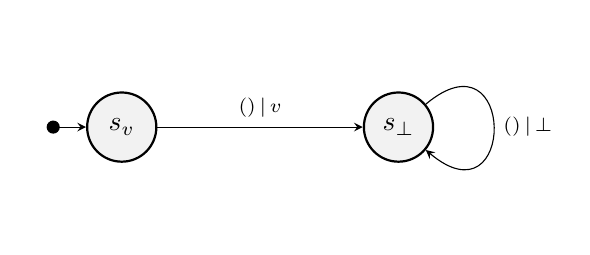
\begin{tikzpicture}[
        ->,
        >=stealth,
        node distance=0.25cm,
        every node/.style={font=\scriptsize},
        every state/.style={font=\normalsize, thick, fill=gray!10},
        initial text=$ $,
        initial distance=0.5cm,
        every initial by arrow/.style={*->},
        x=20pt,
        y=20pt
    ]
    \node[state, initial] (v) at (0,0) {\(s_v\)};
    \node[state] (bot) at (5,0) {\(s_\bot\)};

    \draw (v) edge[above] node{\( () \,|\, v\)} (bot);
    \draw (bot) edge[loop right, out=40, in=320, distance=1.5cm] node{\( () \,|\, \bot\)} (bot);
\end{tikzpicture}
\end{document}